% !TEX root = ../diz.tex
\begin{veta}
  Any maximal parallel P system with cooperative rules without dissolution can be simulated by a sequential P system with cooperative rules and inhibitors.
\end{veta}

\begin{dokaz}
  We show that we can simulate a step of the maximal parallel P system with several steps of a sequential P system with inhibitors.

  % Membrane states

  It is important to note that in the maximal parallel step the evolution occurs simultaneously in all membranes, so we need to synchronize this process.
  The steps of the sequential P system simulating the maximal parallel step are divided into several phases. Every membrane will have a phase, represented as an object. There is exactly one phase object in each membrane. 

  The $\mathit{RUN}$ phase represents that the rules of the maximal parallel P system are being applied, one-by-one. When there are no more rules to apply, the membrane has done its maximal parallel step and proceeds to the phase $\mathit{SYNCHRONIZE}$. Other phases are just technical - we need to implement sending objects between membranes and preparing for the next maximal parallel step by unmarking newly created objects in the current maximal parallel step, which have been marked to prevent double evolution in one step.

  \begin{itemize}
    \item $\mathit{\bf RUN}$: Rules of the maximal parallel P system are being applied. Products are marked ($a^\prime$ instead of $a$) in order to prevent further evolution in the same maximal parallel step. Objects that are to be sent to the parent membrane are directly sent because the parent membrane is in $\mathit{RUN}$ or $\mathit{SYNCHRONIZE}$ phase (see figure \ref{fig:possible_pairs_of_states_of_parent_and_child_membrane}), so the $a^{\prime}$ symbols that are sent will not be used in any rule until phase $\mathit{RESTORE}$. But objects that are to be sent down, cannot be sent immediately because child membranes can be in the previous phase waiting to restore symbols from previous step. Objects $a^\prime$ could interfere with them resulting in double application in current maximal parallel step. Such objects are only marked as $a^{\downarrow\prime}$ to be sent down in the phase $\mathit{SENDDOWN}$. When the phase $\mathit{RUN}$ ends, next phase $\mathit{SYNCHRONIZE}$ takes place, while emitting an object $\mathit{SYNCTOKEN}$ to the parent membrane with a purpose to deliver it to the skin membrane.

    \item $\mathit{\bf SYNCHRONIZE}$: There was no applicable rule left so the membrane is waiting to get signal $\mathit{SYNCED}$ from the parent membrane to proceed to the next phase. And also resending all $\mathit{SYNCTOKEN}$ objects to the parent membrane.

    \item $\mathit{\bf SENDDOWN}$: Signal $\mathit{SYNCED}$ was caught, which means that every membrane has already been in the $\mathit{SYNCHRONIZE}$ phase. And all descendant membranes are in $\mathit{SYNCHRONIZE}$ phase. In this phase all the objects $a^{\downarrow\prime}$ can be sent down.

    \item $\mathit{\bf RESTORE}$: All $a^{\prime}$ symbols are being restored to $a$, preparing for the next maximal parallel step.
  \end{itemize}

  % Rewriting rules

  We will now define the evolution rules of the simulating P system.

  \begin{itemize}
    \item For every rule $r_i\in R$ such that
      \begin{align*}
        r_i = a_1^{M(a_1)}a_2^{M(a_2)}\dots a_n^{M(a_n)} \rightarrow a_1^{N(a_1)}a_2^{N(a_2)}\dots a_n^{N(a_n)}
      \end{align*}
      we will have the following rules:
      \begin{align*}
        &a_1^{M(a_1)-m_1}\dot{a}_1^{m_1}
        a_2^{M(a_2)-m_2}\dot{a}_2^{m_2}\dots
        a_n^{M(a_n)-m_n}\dot{a}_n^{m_n}|\mathit{RUN} \\
        \rightarrow &a_1^{\prime N(a_1)}a_2^{\prime N(a_2)}\dots a_n^{\prime N(a_n)}|\mathit{RUN}
      \end{align*}
      
      There will be such rule for each $0\leq m_i\leq M(a_i)$. It represents the idea that $\dot{a}$ can be used in rewriting in the same way as $a$. Right side of the rules contains symbols $a^\prime$, that prevents the symbols to be rewritten again.

    \item For every symbol $a\in V$, in order to guarantee at most one occurence of $\dot{a}$ in a membrane, we will have the following rules:

    $a|\mathit{RUN} \rightarrow \dot{a}|\mathit{RUN}|_{\neg \dot{a}}$

    \item For every rule $r_i\in R$ there will be a rule that detects if the rule $r_i$ is not applicable. According to left side of the rule $r_i$, symbol $\mathit{UNUSABLE_i}$ will be created when there is not enough objects to fire the rule $r_i$. It means that left side of rule $r_i$ requires more instances of some object than are present in membrane.

    If the left side is of type:
    \begin{itemize}
      \item $a$: It is a context free rule. The rule can't be used if there is no occurrence of $a$ nor $\dot{a}$.

      $\mathit{RUN} \rightarrow \mathit{UNUSABLE_i}|\mathit{RUN}|_{\neg\{\mathit{UNUSABLE_i}, a, \dot{a}\}}$

      \item $ab$: It is a cooperative rule with two distinct objects on the left side. The rule cannot be used if there is one of them missing.

      $\mathit{RUN} \rightarrow \mathit{UNUSABLE_i}|\mathit{RUN}|_{\neg\{\mathit{UNUSABLE_i}, a, \dot{a}\}}$

      $\mathit{RUN} \rightarrow \mathit{UNUSABLE_i}|\mathit{RUN}|_{\neg\{\mathit{UNUSABLE_i}, b, \dot{b}\}}$

      \item $a^2$: It is a cooperative rule with two same objects. The rule can't be used if there is at most one occurrence of the symbol. That happens if there is no occurrence of $a$. There can still be $\dot{a}$, but at most one occurrence.

      $\mathit{RUN} \rightarrow \mathit{UNUSABLE_i}|\mathit{RUN}|_{\neg\{\mathit{UNUSABLE_i}, a\}}$
    \end{itemize}

    \item For every membrane with label $i$ there will be a rule:
    \begin{align*}
      &\mathit{UNUSABLE_1}|\mathit{UNUSABLE_2}|\dots|\mathit{UNUSABLE_m}|\mathit{RUN} \\
      \rightarrow &\mathit{SYNCHRONIZE}|\mathit{SYNCTOKEN_i}\uparrow
    \end{align*}

    If no rule can be used, maximal parallel step in the region is completed hence it goes to the synchronization phase and sends a synchronization token to the parent membrane.

    \item For every membrane there will be a rule:
    \begin{align*}
      &\mathit{SYNCHRONIZE}|\mathit{SYNCTOKEN_j} \\
      \rightarrow &\mathit{SYNCHRONIZE}|\mathit{SYNCTOKEN_j}\uparrow
    \end{align*}

    Membrane resends all synchronization tokens from child membranes to the parent membrane.

    \item In the skin membrane there is a rule which collects all the synchronization tokens from all membranes $1\dots k$ and then sends down signal that synchronization is complete. But before that, there can be some symbols that should be sent down, but they weren't, because the region below could have not started the rewriting phase that time. The result was just marked with $a^{\downarrow\prime}$.
    \begin{align*}
      &\mathit{SYNCTOKEN_1}|\dots|\mathit{SYNCTOKEN_k}|\mathit{SYNCHRONIZE} \\
      \rightarrow &\mathit{SENDDOWN}
    \end{align*}

    \item Every membrane other than skin membrane have to receive the signal to go to the senddown phase:

    $\mathit{SYNCHRONIZE}|\mathit{SYNCED} \rightarrow \mathit{SENDDOWN}$

    \item Every membrane will have rules for every symbol $a\in V$ to send down all unsent objects that should have been sent down:

    $\mathit{SENDDOWN}|a^{\downarrow\prime} \rightarrow \mathit{SENDDOWN}|a^{\prime}\downarrow$

    \item Every membrane will have a rule for detecting when all such objects have been sent and it goes to restore phase:

    $\mathit{SENDDOWN} \rightarrow \mathit{RESTORE}|_{\neg \{a_i^{\downarrow\prime}|1\leq i\leq n\}}$

    \item In the restore phase all symbols $a^{\prime}$ will be rewritten to $a$ in order to be able to be rewritten in the next maximal parallel step:

    $\mathit{RESTORE}|a^{\prime} \rightarrow \mathit{RESTORE}|a$

    \item When the restore phase ends, it sends down a signal that all membranes have been already synchronized and next phase of rewriting has began in upper membranes:

    $\mathit{RESTORE} \rightarrow \mathit{RUN}|\mathit{SYNCED}\downarrow|_{\neg \{a_i^{\prime}|1\leq i\leq n\}}$
  \end{itemize}

  \definecolor{run}{rgb}{1,0.5,0}
  \definecolor{restore}{rgb}{0,0.5,0}
  \definecolor{synchronize}{rgb}{0,0,1}
  \definecolor{senddown}{rgb}{1,0,0}
  % Narrow texts in boxes
  \providecommand{\narrow}[1]{\scalebox{.85}[1.0]{#1}}

  \begin{figure}
    \def\svgwidth{\textwidth}
    \input{possible_pairs_of_states_of_parent_and_child_membrane.pdf_tex}
    % 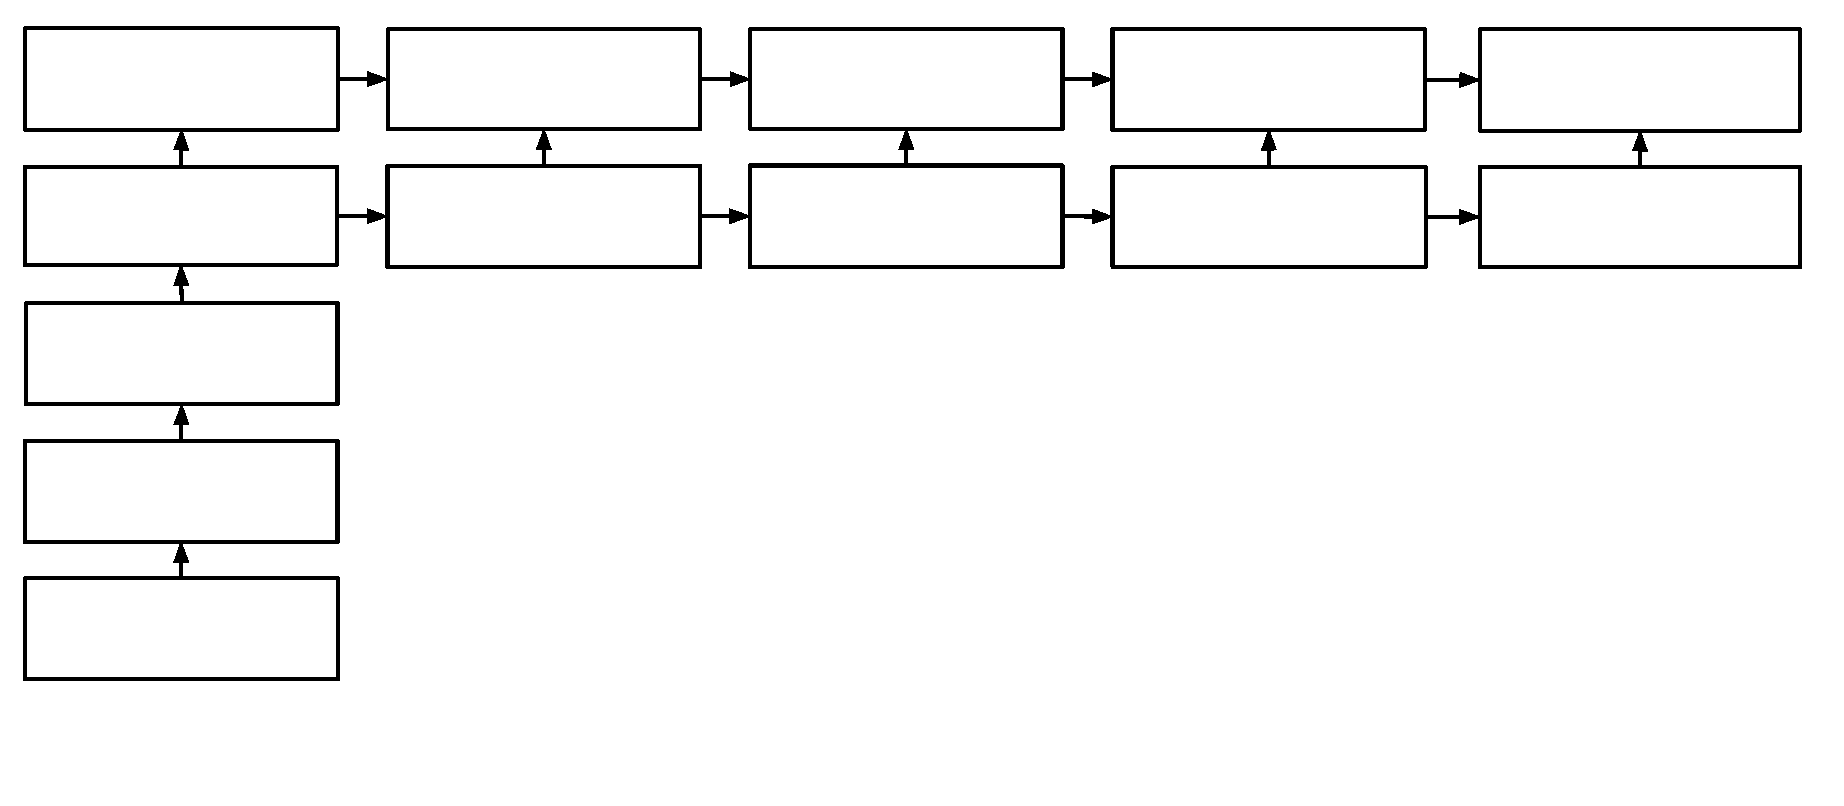
\includegraphics[width=\textwidth]{possible_pairs_of_states_of_parent_and_child_membrane}
    \caption{Possible pairs of states of parent and child membrane}
    \label{fig:possible_pairs_of_states_of_parent_and_child_membrane}
  \end{figure}

  \begin{figure}
    \def\svgwidth{\textwidth}
    \input{snapshot_of_all_membrane_states_while_simulating.pdf_tex}
    % 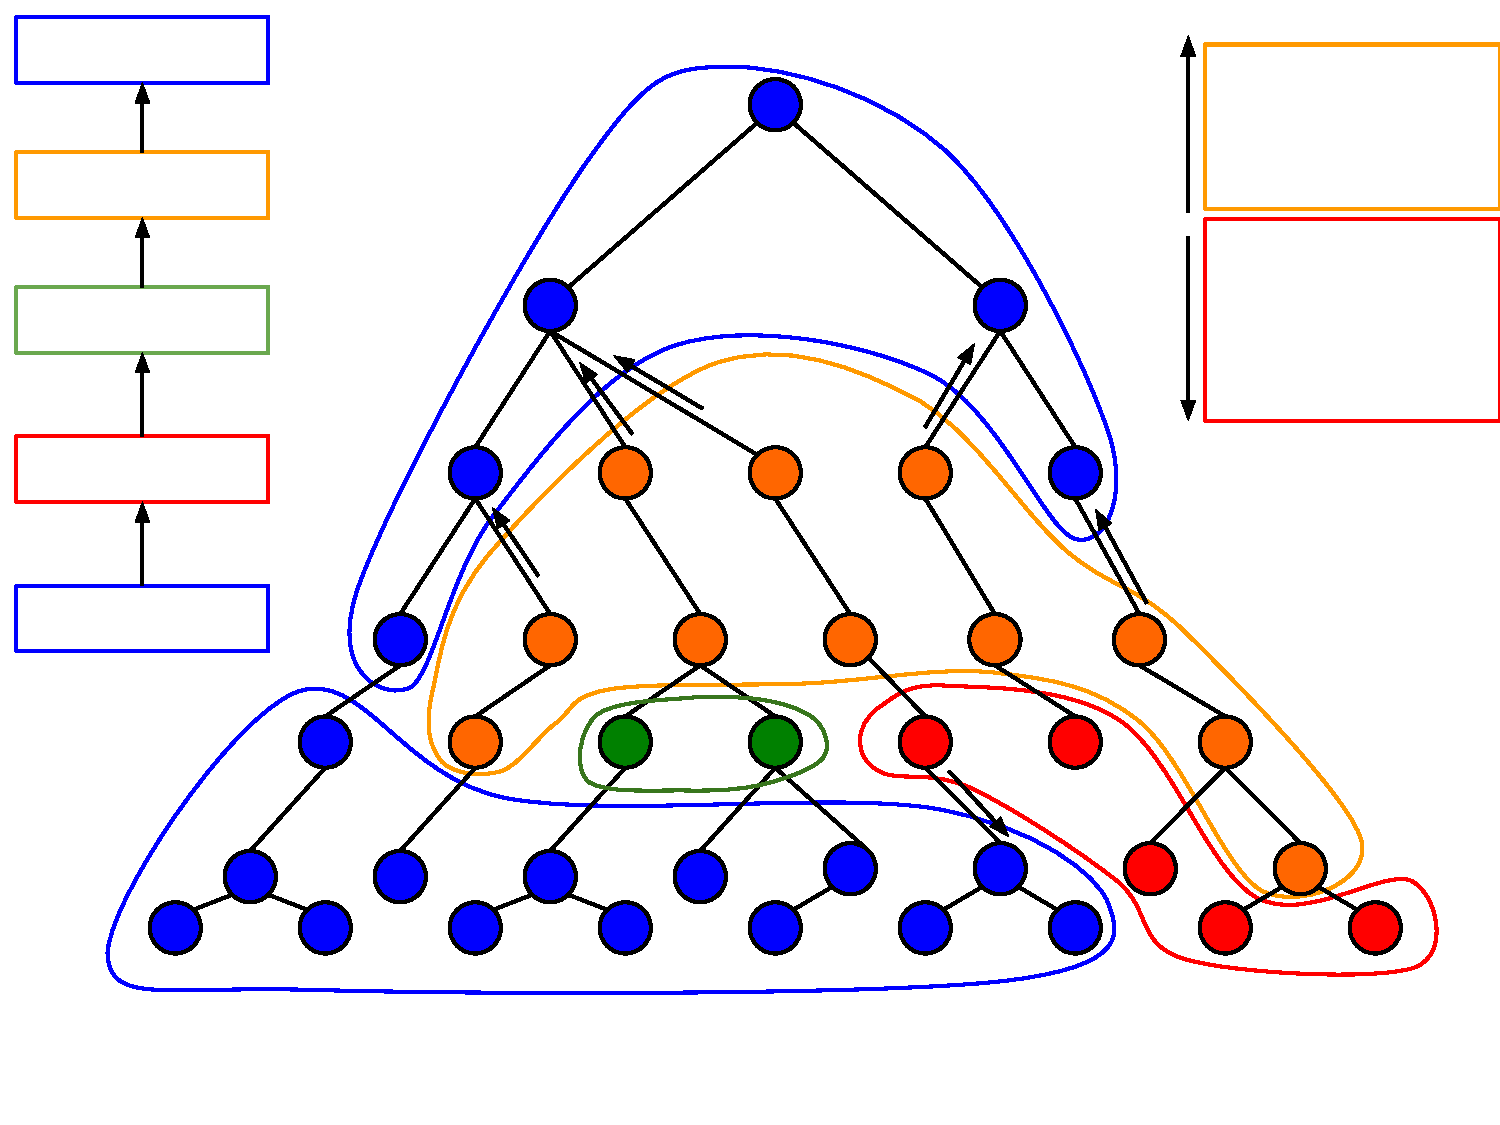
\includegraphics[width=\textwidth]{snapshot_of_all_membrane_states_while_simulating}
    \caption{Snapshot of all membrane states while simulating}
    \label{fig:snapshot_of_all_membrane_states_while_simulating}
  \end{figure}

  The pairs of possible phases of the parent and child membrane are shown in the figure \ref{fig:possible_pairs_of_states_of_parent_and_child_membrane} along with transitions between two consecutive global synchronizations - after the maximal parallel steps $i$ and $i+1$.

  In the figure \ref{fig:snapshot_of_all_membrane_states_while_simulating} the membrane structure is presented as a hierarchical structure. Every membrane is in one of four phases. It can be seen that the sending of the objects is performed in such phases that the receiving membrane is in either $\mathit{RUN}$ or $\mathit{SYNCHRONIZE}$ phase, so the received objects (marked $a^\prime$) does not interfere with rewriting.

  Another interesting idea can be seen in the figure \ref{fig:snapshot_of_all_membrane_states_while_simulating} that when a region is in the $\mathit{SENDDOWN}$ phase and objects are sent through the child membrane, the receiving region is in the $\mathit{SYNCHRONIZE}$ phase waiting for the $\mathit{SYNCED}$ signal, which will be sent to it when $\mathit{SENDDOWN}$ and $\mathit{RESTORE}$ phases finished. \qed

\end{dokaz}
